\chapter{Related Work}\label{chap:related-work}
Hauder et al. mention numerous research challenges in the domain of ACM, among them an active support system for knowledge workers \cite{hauder2014}.
The need for such a system is emphasized by Francescomarino et al. in an extensive literature review, where it has been found that few prediction approaches target the next activity \cite{francescomarino2018}.\\

This evident lack in this area has motivated this thesis. As shown in the previous chapters, it brings the domains of process science and data science together. In both, research has been published on sequence prediction. In the former in the context of processes and events and in the latter in the context of text modeling and NLP. Seperated by domain, the related works in these domains shall be presented in this chapter.

\section{Process prediction}
\marginpar{CoCaMa is an abbreviation for a project called Collaborative Case Management that appears to be retired: \href{http://archive.li/uZFnN}{archive.li/uZFnN}}
An example for how a support system \cite{hauder2014} for case workers might look like is given by Huber, who has developed a next-step prediction and recommendation system  \cite{huber2015}. The system is prototypically implemented within CoCaMa, a case management application.

After gathering the training data from various sources via an extract, transform and load (ETL) process, several \textit{Next Models} are constructed. The Next Models are a collection of predictive models used to predict the next activity, focused on different criteria: remaining time, constraint violation, decisions based on case-specific data, and case outcome. The weighting of the predictions from these individual models is non-trivial and extensively discussed. Huber models the prediction as a classification problem and uses decision trees from the WEKA \cite{web:weka} machine learning toolkit to implement them. The system has been evaluated with 25 hand-made case logs \cite{huber2015}.\\

Building upon each other are the works by Evermann et al. \cite{evermann2016} and Schönig et al. \cite{schoenig2018}. Evermann et al. remark the lack of research on next event predictions and have successfully demonstrated the applicability of LSTM neural networks in the context of predicting the next activity. Using a neural network implemented with Tensorflow, precisions between $60\%$ to $90\%$ on the BPIC2012 and BPIC2013 datasets are achieved. Evermann et al. want their work to be understood as a "demonstration of the applicability of the approach and the potential for future work". The authors highlight that their work lacks use of data attributes during model training.

Schönig et al. \cite{schoenig2018} picked up on Evermann's future work and demonstrated on BPIC datasets from 2017 that using data attributes does increase prediction accuracy. Schönig et al. implemented their solution with Keras and trained it using stratified 5-fold cross-validation. Their data was preprocessed with one-hot encoding for categorical variables and min-max-normalization for continuous features. Also, the work nicely demonstrates that an increasing number of included data attributes can continually improve accuracy \cite[p.5]{schoenig2018}, without referring to any of their statistical properties.

The works of Evermann et al. and Schönig et al. represent important parts of Contribution and Evaluation, as they are similar to our approach and the source code for both works has been made available.\\

Similar to Schönig et al., Polato et al. make use of data attributes in their work for improving the prediction of the remaining time of business process instances \cite{polato2014}. During feature engineering, their SVR training data is enriched with information about possible other activities. Their dataset is unfortunately relatively small at 5000 items and not public.\\

Metzger et al. predict constraint violation of a case by comparing fundamentally different prediction models and combining them into a model ensemble based on various criteria \cite{metzger2015}. They argue that late and precise or early and incorrect predictions are both worthless for interventions, leading them to establish that between $60\% - 85\%$ progress into the process, predictions become stable and precise.

Three models are used to predict constraint violations: constraint satisfaction, Quality-of-Service (QoS) violation checks and machine learning. The two former models use rules to predict a process outcome while the latter is a trained neural network. For it, Metzger et. al use the ANN implementation from the WEKA machine learning toolkit with a single hidden layer. 

The authors are able to formulate rules for the two other models because the process at hand is very rigid and well defined: The Cargo 2000 process is a standard proposed by the International Air Transport Association (IATA) \cite{metzger2015}.\\

Also aiming at predicate fulfilment were Francescomarino et al. when they they organized predictive models in a clustered fashion \cite{francescomarino2015}. Having clustered the training data, one model was trained on each cluster. Then, to obtain a prediction, the cluster for a new data item needs to found, and the corresponding model selected. Furthermore, the authors varied the probability threshold for accepting a prediction and measured how it affected the point at which the predictions become stable (similar to Metzger et al.). They referred to this characteristic as \textit{earliness}. Their approach, implemented as a ProM plugin called \textit{Predictive Process Monitoring.}, uses two different clustering methods (k-means and DBSCAN) and two different types of predictive models (decision trees and random forests). It was tested on the BPIC2011 dataset \cite{BPIC2011} without emphasis on hyperparameter tuning.

Picking up on Francescomarinos approach and training a neural network for every cluster was heavily considered at the beginning of this thesis but foregone because of the possibility to use embedding layers which cause clustering inside the ANN.\\

Klinkmüller et al. enrich their training dataset with markers that encode subsequence occurrence \cite{klinkmuller2018reliablemonitoring}. Doing so on a synthetic and undisclosed dataset, they are able to increase the accuracy of a random forest in comparison to a baseline that is not using the engineered subsequence features. This approach is similar to that of Shibata et al. \cite{shibata2016bipartite} two years earlier.\\

Approaching the process prediction in a different fashion are Böhmer et al. with predictions rooted in heuristic analysis \cite{boehmer2018probability}. Based on the fact that the black-box nature of ANNs makes their predictions and inner workings very hard to comprehend, they argue that the amount of trust that users put into their predictions results is limited. As potentially large organizational changes could be made due to the predictions, the authors perceive it of importance to explain alternative futures which were not classified as being most probable and explain the aspects which motivated specific prediction results.
Böhmer et al. approximate trace similarities with the Damerau-Levenstein method and a custom cost function. Using this method, they filter historic traces to produce a set of similar executions. From this set, probability distributions are mined, with the most probable behaviour ultimately used as the final prediction \cite{boehmer2018probability}.

\section{Text modeling}
Colocated with the International Conference in Grammatical Inference 2016 (ICGI) was a competition called SPiCE\ "about guessing the next element in a sequence" \cite{web:spice}. Most entries submitted to this competition made use of RNNs with LSTM cells to predict the next word of a sentence.

\begin{figure}
    \centering
    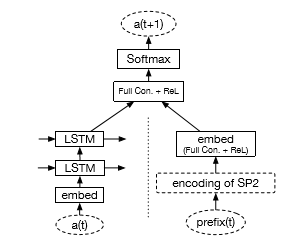
\includegraphics[height=.4\textwidth]{gfx/spice-winner-architecture.png}
    \caption{The neural network architecture of the winning submission at the SPiCE competition by Shibata et al. \cite{shibata2016bipartite}.}
    \label{fig:spice-winner-architecture}
\end{figure}

The winning submission by Shibata et al. uses a bipartite network architecture training separate layers on different features of the same sentence. The results of these separate layers are then merged in the middle hidden layers to produce a single output \cite{shibata2016bipartite}, as \autoref{fig:spice-winner-architecture} shows.
While one half of the layers are trained on the most recent word of the sentence, the other half is trained on the prefix of that word. As this prefix can be of any length, Shibata et al. propose a binary bag-of-words encoding, representing the states of a SP-2 automaton.

SP-$k$ languages are used to describe certain long-term dependencies through forbidden subsequences. For example, if $\langle a,b \rangle$ is forbidden, then no $b$ may ever occur after $a$. As per Heinz, who assisted Shibata, deterministic finite automatons (DFA) can also be used to characterize SP-$k$ languages, if its states encode the subsequences of size $k-1$  present in the previous prefixes \cite{heinz2010estimatingSP}. To make this concept more tangible, \autoref{tab:sp2-encoding} illustrates a small example.

\begin{table}[ht!]
    \centering
    \begin{tabular}{cclccccc}
        \hline
          &      &              & \multicolumn{5}{c}{SP-2 vector}\\
        t & a(t) & prefix(a(t)) & [a & b & c & d & e]\\
        \hline
        0 & a    & a            & [1 & 0 & 0 & 0 & 0]\\
        1 & d    & ad           & [1 & 0 & 0 & 1 & 0]\\
        2 & a    & ada          & [1 & 0 & 0 & 1 & 0]\\
        % 3 & c    & adac         & [1 & 0 & 1 & 1 & 0]\\
        % 4 & d    & adacd        & [1 & 0 & 1 & 1 & 0]\\
        \hline
    \end{tabular}
    \caption{Prefixes encoded with SP-2. As $t$ progresses, more and more single-item subsequences ($k-1=1$) are marked as occurred. The alphabet is $I=\{a,b,c,d,e\}$. This example is taken from Shibata et al.  \cite{shibata2016bipartite}.}
    \label{tab:sp2-encoding}
\end{table}

Attention, a fairly new development in the domain of ANNs, has been leveraged by Kokkinos et al. in a tree-structured neural network to classify sentiments in sentences \cite{kokkinos2017structural}. In a detailed comparison with other works, their bipartite tree approach yields the highest accuracy on the Stanford Sentiment Treebank dataset. While the proposition of tree-structured Gated Recurrent Units (GRUs, a variant of LSTM units) and their use of attention is arguably the main contribution of this work, they make use of a bipartite network architecture and word embeddings as well.